


\title{RcppOctave: Octave along with R}  %% just a draft title
\author{by Renaud Gaujoux and Dirk Eddelbuettel}

\maketitle

\abstract{
  The \pkg{RcppOctave} package connects Octave to R. TODO: Expand
}

\section{Introduction}

Octave \citep{Eaton:2008} is a high-level interactive language which is
primarily intended for numerical computations.  It has found widespread
adoption across different disciplines as it is mostly compatible with Matlab
\citep{MATLAB:2010}.  While Matlab has historically been pre-eminent in
domains such as applied mathematics, electrical engineering and signal
processing, it is also widely used in other fields such as machine
learning, %% TODO/DE: Maybe ask Soren and the folks at MLOSS.org about Matlab numbers
bioinformatics, and finance.  Consequently, a large corpus of application
programs are available as \code{.m}-files (named after the commonly-chose
file extension) for which Octave provides an open source engine.

R \citep{R:2012}, a language and environment for statistical
computing and graphics, has become the dominant language for statistical
research, and a widely-used environment for empirical work in a variety of
fields. % DE: I don't want to single out BioC here, but maybe we could point
        % to the CRAN Task Views? Or just leave it as this is for the R Journal..

While both languages share commonalities, their respective focus is different
making a combination of both environments an even more compelling choice.
This short paper illustrates the \pkg{RcppOctave} package by
\cite{CRAN:RcppOctave} which implements an interface between both these
environments.

\section{Octave}

TODO: Two or three short paragraphs about Octave

\section{Example: Matrix Operations}  % or something else

TODO: Show two or three simple call illustrating the variable arguments etc.

\section{Example: Kalman Filter}

\cite{Eddelbuettel+Sanderson:2012} motivate the \pkg{RcppArmadillo} package
with an example comparing a Kalman Filter implementation in both R and
C++. As the code underlying this example was initially published for
Matlab\footnote{See
  \url{http://www.mathworks.com/products/matlab-coder/demos.html?file=/products/demos/shipping/coder/coderdemo_kalman_filter.html}.},
it can of course also be used with RcppOctave.

TODO: Few words about the example

TODO: render code 'pretty' whith knitr which must have a Matlab filter too

\noindent
\ttfamily
\hlstd{}\hlkwa{function\ }\hlstd{Y\ }\hlopt{=\ }\hlstd{kalmanM}\hlopt{(}\hlstd{pos}\hlopt{)}\hspace*{\fill}\\
\hlstd{}\hlstd{\ \ }\hlstd{dt}\hlopt{=}\hlstd{}\hlnum{1}\hlstd{}\hlopt{;}\hspace*{\fill}\\
\hlstd{}\hlstd{\ \ }\hlstd{}\hlslc{\%\%\ Initialize\ state\ transition\ matrix}\hspace*{\fill}\\
\hlstd{}\hlstd{\ \ }\hlstd{A}\hlopt{={[}\ }\hlstd{}\hlnum{1\ 0\ }\hlstd{dt\ }\hlnum{0\ 0\ 0}\hlstd{}\hlopt{;}\hlstd{...}\hlstd{\ \ \ \ \ }\hlstd{}\hlslc{\%\ {[}x}\hlstd{\ \ }\hlslc{{]}}\hspace*{\fill}\\
\hlstd{}\hlstd{\ \ \ \ \ }\hlstd{}\hlnum{0\ 1\ 0\ }\hlstd{dt\ }\hlnum{0\ 0}\hlstd{}\hlopt{;}\hlstd{...}\hlstd{\ \ \ \ \ }\hlstd{}\hlslc{\%\ {[}y}\hlstd{\ \ }\hlslc{{]}}\hspace*{\fill}\\
\hlstd{}\hlstd{\ \ \ \ \ }\hlstd{}\hlnum{0\ 0\ 1\ 0\ }\hlstd{dt\ }\hlnum{0}\hlstd{}\hlopt{;}\hlstd{...}\hlstd{\ \ \ \ \ }\hlstd{}\hlslc{\%\ {[}Vx{]}}\hspace*{\fill}\\
\hlstd{}\hlstd{\ \ \ \ \ }\hlstd{}\hlnum{0\ 0\ 0\ 1\ 0\ }\hlstd{dt}\hlopt{;}\hlstd{...}\hlstd{\ \ \ \ \ }\hlstd{}\hlslc{\%\ {[}Vy{]}}\hspace*{\fill}\\
\hlstd{}\hlstd{\ \ \ \ \ }\hlstd{}\hlnum{0\ 0\ 0\ 0\ 1\ 0\ }\hlstd{}\hlopt{;}\hlstd{...}\hlstd{\ \ \ \ \ }\hlstd{}\hlslc{\%\ {[}Ax{]}}\hspace*{\fill}\\
\hlstd{}\hlstd{\ \ \ \ \ }\hlstd{}\hlnum{0\ 0\ 0\ 0\ 0\ 1\ }\hlstd{}\hlopt{{]};}\hlstd{\ \ \ \ \ \ \ }\hlopt{}\hlstd{}\hlslc{\%\ {[}Ay{]}}\hspace*{\fill}\\
\hlstd{}\hlstd{\ \ }\hlstd{}\hlslc{\%\ Initialize\ measurement\ matrix}\hspace*{\fill}\\
\hlstd{}\hlstd{\ \ }\hlstd{H\ }\hlopt{=\ {[}\ }\hlstd{}\hlnum{1\ 0\ 0\ 0\ 0\ 0}\hlstd{}\hlopt{;\ }\hlstd{}\hlnum{0\ 1\ 0\ 0\ 0\ 0\ }\hlstd{}\hlopt{{]};}\hspace*{\fill}\\
\hlstd{}\hlstd{\ \ }\hlstd{Q\ }\hlopt{=\ }\hlstd{eye}\hlopt{(}\hlstd{}\hlnum{6}\hlstd{}\hlopt{);}\hspace*{\fill}\\
\hlstd{}\hlstd{\ \ }\hlstd{R\ }\hlopt{=\ }\hlstd{}\hlnum{1000\ }\hlstd{}\hlopt{{*}\ }\hlstd{eye}\hlopt{(}\hlstd{}\hlnum{2}\hlstd{}\hlopt{);}\hspace*{\fill}\\
\hlstd{}\hlstd{\ \ }\hlstd{x\textunderscore est\ }\hlopt{=\ }\hlstd{zeros}\hlopt{(}\hlstd{}\hlnum{6}\hlstd{}\hlopt{,\ }\hlstd{}\hlnum{1}\hlstd{}\hlopt{);}\hspace*{\fill}\\
\hlstd{}\hlstd{\ \ }\hlstd{p\textunderscore est\ }\hlopt{=\ }\hlstd{zeros}\hlopt{(}\hlstd{}\hlnum{6}\hlstd{}\hlopt{,\ }\hlstd{}\hlnum{6}\hlstd{}\hlopt{);}\hspace*{\fill}\\
\hlstd{\hspace*{\fill}\\
}\hlstd{\ \ }\hlstd{numPts\ }\hlopt{=\ }\hlstd{}\hlkwa{size}\hlstd{}\hlopt{(}\hlstd{pos}\hlopt{,}\hlstd{}\hlnum{1}\hlstd{}\hlopt{);}\hspace*{\fill}\\
\hlstd{}\hlstd{\ \ }\hlstd{Y\ }\hlopt{=\ }\hlstd{zeros}\hlopt{(}\hlstd{numPts}\hlopt{,\ }\hlstd{}\hlnum{2}\hlstd{}\hlopt{);}\hspace*{\fill}\\
\hlstd{\hspace*{\fill}\\
}\hlstd{\ \ }\hlstd{}\hlkwa{for\ }\hlstd{idx\ }\hlopt{=\ }\hlstd{}\hlnum{1}\hlstd{}\hlopt{:}\hlstd{numPts\hspace*{\fill}\\
}\hlstd{\ \ \ \ }\hlstd{z\ }\hlopt{=\ }\hlstd{pos}\hlopt{(}\hlstd{idx}\hlopt{,\ :)}\hlstd{'}\hlopt{;}\hspace*{\fill}\\
\hlstd{\hspace*{\fill}\\
}\hlstd{\ \ \ \ }\hlstd{}\hlslc{\%\%\ Predicted\ state\ and\ covariance}\hspace*{\fill}\\
\hlstd{}\hlstd{\ \ \ \ }\hlstd{x\textunderscore prd\ }\hlopt{=\ }\hlstd{A\ }\hlopt{{*}\ }\hlstd{x\textunderscore est}\hlopt{;}\hspace*{\fill}\\
\hlstd{}\hlstd{\ \ \ \ }\hlstd{p\textunderscore prd\ }\hlopt{=\ }\hlstd{A\ }\hlopt{{*}\ }\hlstd{p\textunderscore est\ }\hlopt{{*}\ }\hlstd{A'\ }\hlopt{+\ }\hlstd{Q}\hlopt{;}\hspace*{\fill}\\
\hlstd{}\hlstd{\ \ \ \ }\hlstd{}\hlslc{\%\%\ Estimation}\hspace*{\fill}\\
\hlstd{}\hlstd{\ \ \ \ }\hlstd{S\ }\hlopt{=\ }\hlstd{H\ }\hlopt{{*}\ }\hlstd{p\textunderscore prd'\ }\hlopt{{*}\ }\hlstd{H'\ }\hlopt{+\ }\hlstd{R}\hlopt{;}\hspace*{\fill}\\
\hlstd{}\hlstd{\ \ \ \ }\hlstd{B\ }\hlopt{=\ }\hlstd{H\ }\hlopt{{*}\ }\hlstd{p\textunderscore prd'}\hlopt{;}\hspace*{\fill}\\
\hlstd{}\hlstd{\ \ \ \ }\hlstd{klm\textunderscore gain\ }\hlopt{=\ (}\hlstd{S\ $\backslash$\ B}\hlopt{)}\hlstd{'}\hlopt{;}\hspace*{\fill}\\
\hlstd{}\hlstd{\ \ \ \ }\hlstd{}\hlslc{\%\%\ Estimated\ state\ and\ covariance}\hspace*{\fill}\\
\hlstd{}\hlstd{\ \ \ \ }\hlstd{x\textunderscore est\ }\hlopt{=\ }\hlstd{x\textunderscore prd\ }\hlopt{+\ }\hlstd{klm\textunderscore gain\ }\hlopt{{*}\ (}\hlstd{z\ }\hlopt{{-}\ }\hlstd{H\ }\hlopt{{*}\ }\hlstd{x\textunderscore prd}\hlopt{);}\hspace*{\fill}\\
\hlstd{}\hlstd{\ \ \ \ }\hlstd{p\textunderscore est\ }\hlopt{=\ }\hlstd{p\textunderscore prd\ }\hlopt{{-}\ }\hlstd{klm\textunderscore gain\ }\hlopt{{*}\ }\hlstd{H\ }\hlopt{{*}\ }\hlstd{p\textunderscore prd}\hlopt{;}\hspace*{\fill}\\
\hlstd{}\hlstd{\ \ \ \ }\hlstd{}\hlslc{\%\%\ Compute\ the\ estimated\ measurements}\hspace*{\fill}\\
\hlstd{}\hlstd{\ \ \ \ }\hlstd{Y}\hlopt{(}\hlstd{idx}\hlopt{,\ :)\ =\ }\hlstd{H\ }\hlopt{{*}\ }\hlstd{x\textunderscore est}\hlopt{;}\hspace*{\fill}\\
\hlstd{}\hlstd{\ \ }\hlstd{}\hlkwa{end}\hlstd{\ \ \ \ \ \ \ \ \ \ \ \ \ \ \ \ }\hlkwa{}\hlstd{}\hlslc{\%\ of\ the\ function}\hspace*{\fill}\\
\hlstd{}\hlkwa{end}\hlstd{\ \ \ }\hlkwa{}\hlstd{}\hlslc{\%\ of\ the\ function}\hlstd{}\hspace*{\fill}\\
\mbox{}
\normalfont
\normalsize



This function, along with several R implementations, is provided in the
\pkg{RcppOctave} package as \code{demo(Kalman)}. % TODO: just a suggestion
Table~\ref{tab:benchmark} summaries the performance.

%                 test replications elapsed relative
% 7  KalmanOctave(pos)          100   3.943  1.00000
% 2      KalmanRC(pos)          100   5.987  1.51839
% 1       KalmanR(pos)          100   6.047  1.53360
% 4   KalmanRfunC(pos)          100   6.262  1.58813
% 3    KalmanRfun(pos)          100   6.648  1.68603
% 6 FirstKalmanRC(pos)          100   8.992  2.28050
% 5  FirstKalmanR(pos)          100   9.405  2.38524

\begin{table}[hbt]
  \begin{center}
    \begin{small}
      \begin{tabular}{lrr}
        \toprule
        {\bf Implementation \phantom{XX}} & {\bf Time in sec.} & {\bf Rel.~ to best} \\
        \cmidrule(r){1-3}
         KalmanOctave  & 3.943 & 1.000 \\
             KalmanRC  & 5.987 & 1.518 \\
              KalmanR  & 6.047 & 1.534 \\
          KalmanRfunC  & 6.262 & 1.588 \\
           KalmanRfun  & 6.648 & 1.686 \\
        FirstKalmanRC  & 8.992 & 2.281 \\
         FirstKalmanR  & 9.405 & 2.385 \\
        \bottomrule
      \end{tabular}
      \caption{Performance comparison of various implementations of a Kalman filter.
        KalmanOctave is the \pkg{RcppOctave} based implementation shown above.
        KalmanR is the \R implementation using an environment; KalmanRfun use a
        function; FirstKalmanR is a direct translation of the original Matlab
        implementation; versions ending in C are the byte-compiled variants of
        the respective version.  Timings are averaged over 100 replications.
        The comparison was made using R version 2.15.1, Rcpp version 0.9.13 and
        RcppOctave version 0.8.5 on Ubuntu 12.04 running in 64-bit mode on a
        2.67 GHz Intel i7 processor.}
      \label{tab:benchmark}
    \end{small}
  \end{center}
\end{table}

% TODO: We may want to skip one (pair) of the R variants...

TODO: More about the example, performance comparison, knocking socks off R


\section{Example: Gibbs Sampler}

Wilkinson (TODO: Reference from his repeated blog posts) used a simple
bivariate Gibbs Sampler as a basis for comparisons between different
programming languages such as C, Java, Python and R. His example has been
re-used in number of other presentations.

We can adapt this example here as it provides a suitable framework for
showing how \pkg{RcppOctave} can interact with the random number generators
in R.

%DE: Super-useful feature, but shall we have that here or as part of the Gibbs sampler comparison
TODO: Make true Gibbs sampler example
\begin{knitrout}
\definecolor{shadecolor}{rgb}{0.933, 0.933, 0.933}\color{fgcolor}\begin{kframe}
\begin{alltt}
\hlfunctioncall{library}(RcppOctave)
\end{alltt}


{\ttfamily\noindent\itshape\color{messagecolor}{\#\# Loading required package: Rcpp}}

{\ttfamily\noindent\itshape\color{messagecolor}{\#\# Loading required package: pkgmaker}}\begin{alltt}

\hlcomment{# R runif}
\hlfunctioncall{set.seed}(1)
a <- \hlfunctioncall{runif}(10)

\hlcomment{# define octave function}
\hlfunctioncall{o_source}(text="
function [x] = \hlfunctioncall{orng}(n)
	x = \hlfunctioncall{rand}(1, n);
end
")
\hlfunctioncall{set.seed}(1)
\hlfunctioncall{identical}(.O$\hlfunctioncall{orng}(10), a)
\end{alltt}
\begin{verbatim}
## [1] TRUE
\end{verbatim}
\begin{alltt}

\hlcomment{## similarly for Gamma:}
\hlfunctioncall{o_source}(text="function [x] = \hlfunctioncall{orngg}(n)
     x = \hlfunctioncall{randg}(1, n);
end
")
\hlcomment{## returns a 500 x 500 matrix}
\hlfunctioncall{set.seed}(42)
\hlcomment{## same as 'lightblue' below so we have  'randg(a, N)/b' == rgamma(a,b)}
\hlfunctioncall{plot}(\hlfunctioncall{density}(\hlfunctioncall{as.vector}(\hlfunctioncall{matrix}(.O$\hlfunctioncall{orngg}(500),ncol=1))/2))
\end{alltt}
\end{kframe}
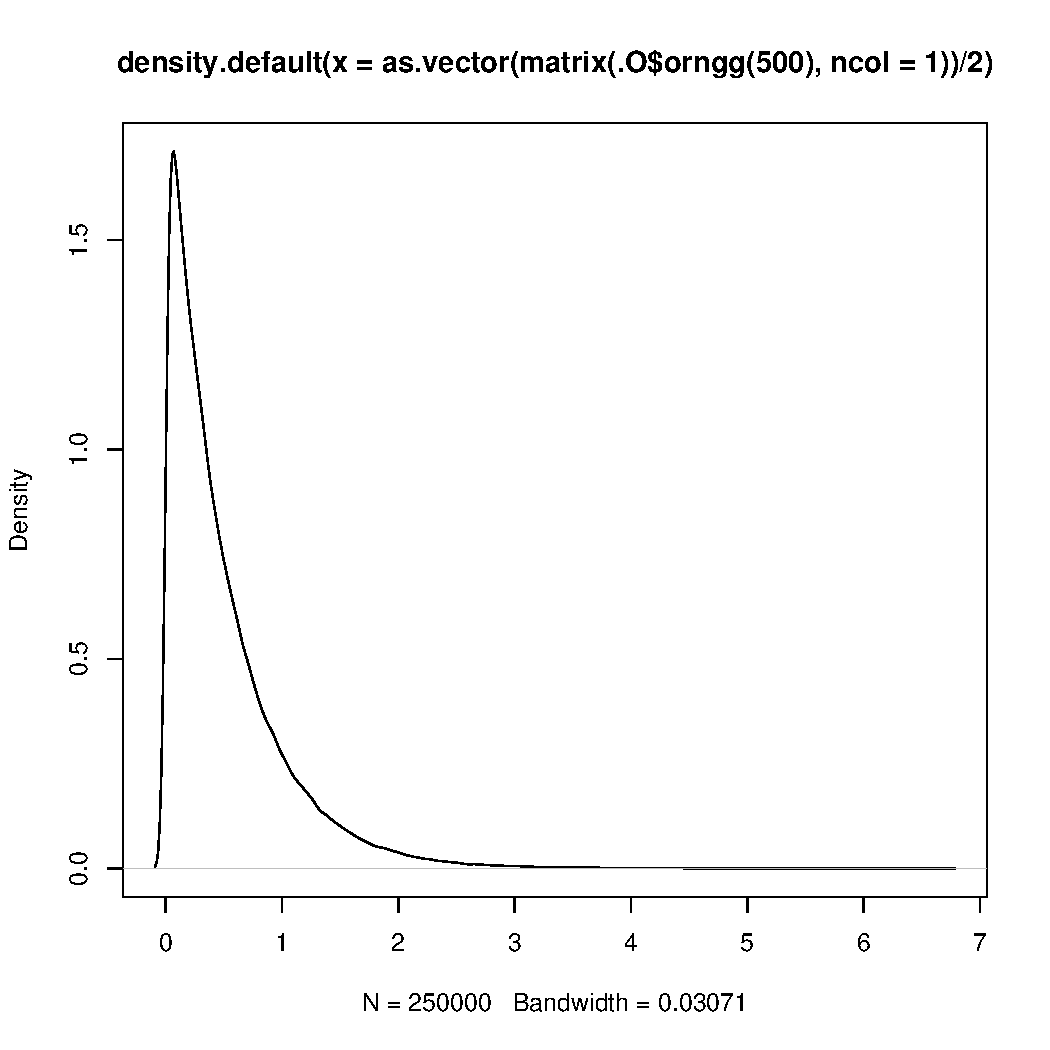
\includegraphics[width=\maxwidth]{/home/renaud/Documents/projects/RcppOctave/pkg/vignettes/figure/RJwrapper-rng1} 
\begin{kframe}\begin{alltt}

\hlcomment{## about the same in R:}
\hlfunctioncall{set.seed}(42)
\hlfunctioncall{plot}(\hlfunctioncall{density}(\hlfunctioncall{rgamma}(25000,1,1)), ylim=\hlfunctioncall{c}(0,1.8))
\hlfunctioncall{lines}(\hlfunctioncall{density}(\hlfunctioncall{rgamma}(25000,1,2)), col=\hlstring{'gray'})
\hlfunctioncall{lines}(\hlfunctioncall{density}(\hlfunctioncall{rgamma}(25000,1,1/2)), col=\hlstring{'lightblue'})
\end{alltt}
\end{kframe}
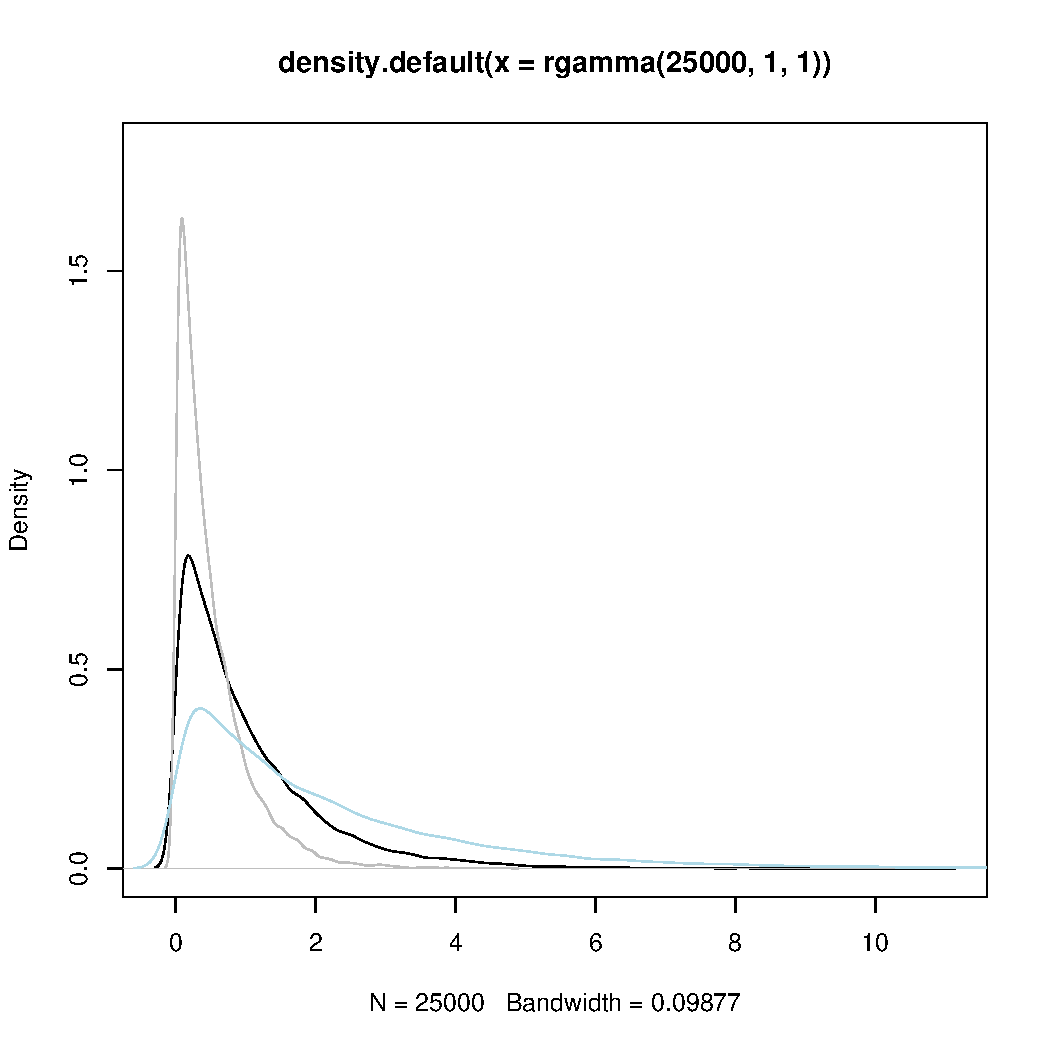
\includegraphics[width=\maxwidth]{/home/renaud/Documents/projects/RcppOctave/pkg/vignettes/figure/RJwrapper-rng2} 

\end{knitrout}



\bibliography{../inst/REFERENCES}


\address{Renaud Gaujoux \\
  Computational Biology \\
  University of Cape Town \\
  Cape Town \\
  South Africa}\\
\email{renaud@cbio.uct.ac.za}

\address{Dirk Eddelbuettel \\
  %Affiliation\\
  River Forest, IL\\
  USA}\\
\email{edd@debian.org}


%%% Local Variables:
%%% mode: latex
%%% TeX-master: "RJwrapper"
%%% End:
